\documentclass[12pt,3p]{article}
\usepackage[margin=0.75in]{geometry}
\usepackage[T1]{fontenc}
\usepackage[utf8]{inputenc}
\usepackage[english]{babel}
\usepackage{amsmath}
\usepackage{mathtools}
\usepackage{enumitem}
\usepackage{physics}
\usepackage{bm}

\usepackage[round,numbers]{natbib}
\usepackage[colorlinks = false]{hyperref}

\hypersetup{
    colorlinks=false, %set true if you want colored links
    linktoc=all,      %set to all if you want both sections and subsections linked
    % linkcolor=blue,  %choose some color if you want links to stand out
}

\begin{document}

\title{\Large{FEniCS: Hyperelastic Formulations} \vspace{-2ex}}
\author{Ida Ang: Edited \today}
\date{\vspace{-5ex}}
\maketitle

\tableofcontents
\newpage

%===============================================================================================
%===============================================================================================
%===============================================================================================
\section{Problem Definition}
\vspace{-2ex}

This document is based on the \href{https://fenicsproject.org/olddocs/dolfin/1.4.0/python/demo/documented/hyperelasticity/python/documentation.html}{FEniCS hyperelasticity demonstration}, which is formulated using the concept of minimization of potential energy. Hyperelastic models are a type of constitutive (stress-strain) model, where the stress and strain are not linearly related as they are in linear elastic models. Hyperelastic constitutive models can be used to describe materials such as rubbers, elastomers, and load bearing musculoskeletal tissues such as cartilage. 

The goal of this document is to 1) provide more details of the theory, and 2) provide an alternate formulation where the strong form, or partial differential equation, is converted to the weak form, or integral equation, and written explicitly. This document provides the detailed steps for beginners who might have just been exposed to continuum mechanics and indicial notation. In direct notation, bolded uncapitalized notation refers to vectors, unbolded notation refers to scalar variables.

The original demonstration involves a three-dimensional cube, where a boundary condition is provided that twists the top part of the cube. See Fig. \ref{FigVisual} for an example of reference and current configuration.
\begin{figure*}[!htb]
\centering
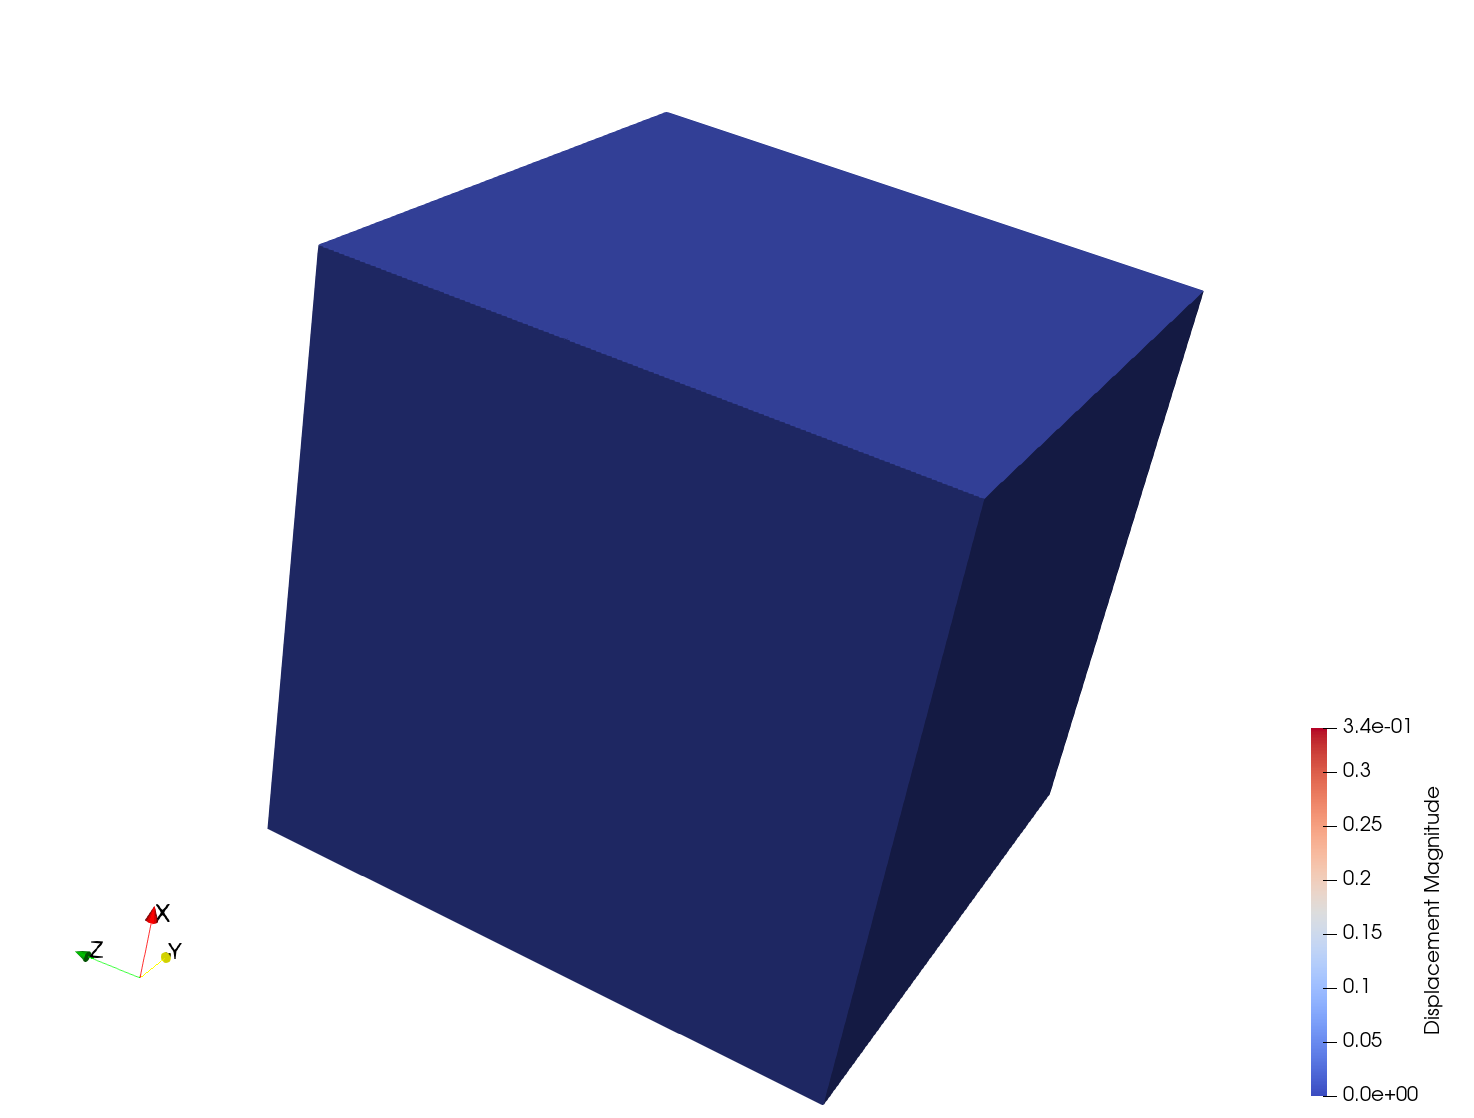
\includegraphics[width=0.49\textwidth]{./Images/MixedForm/Disp_00}
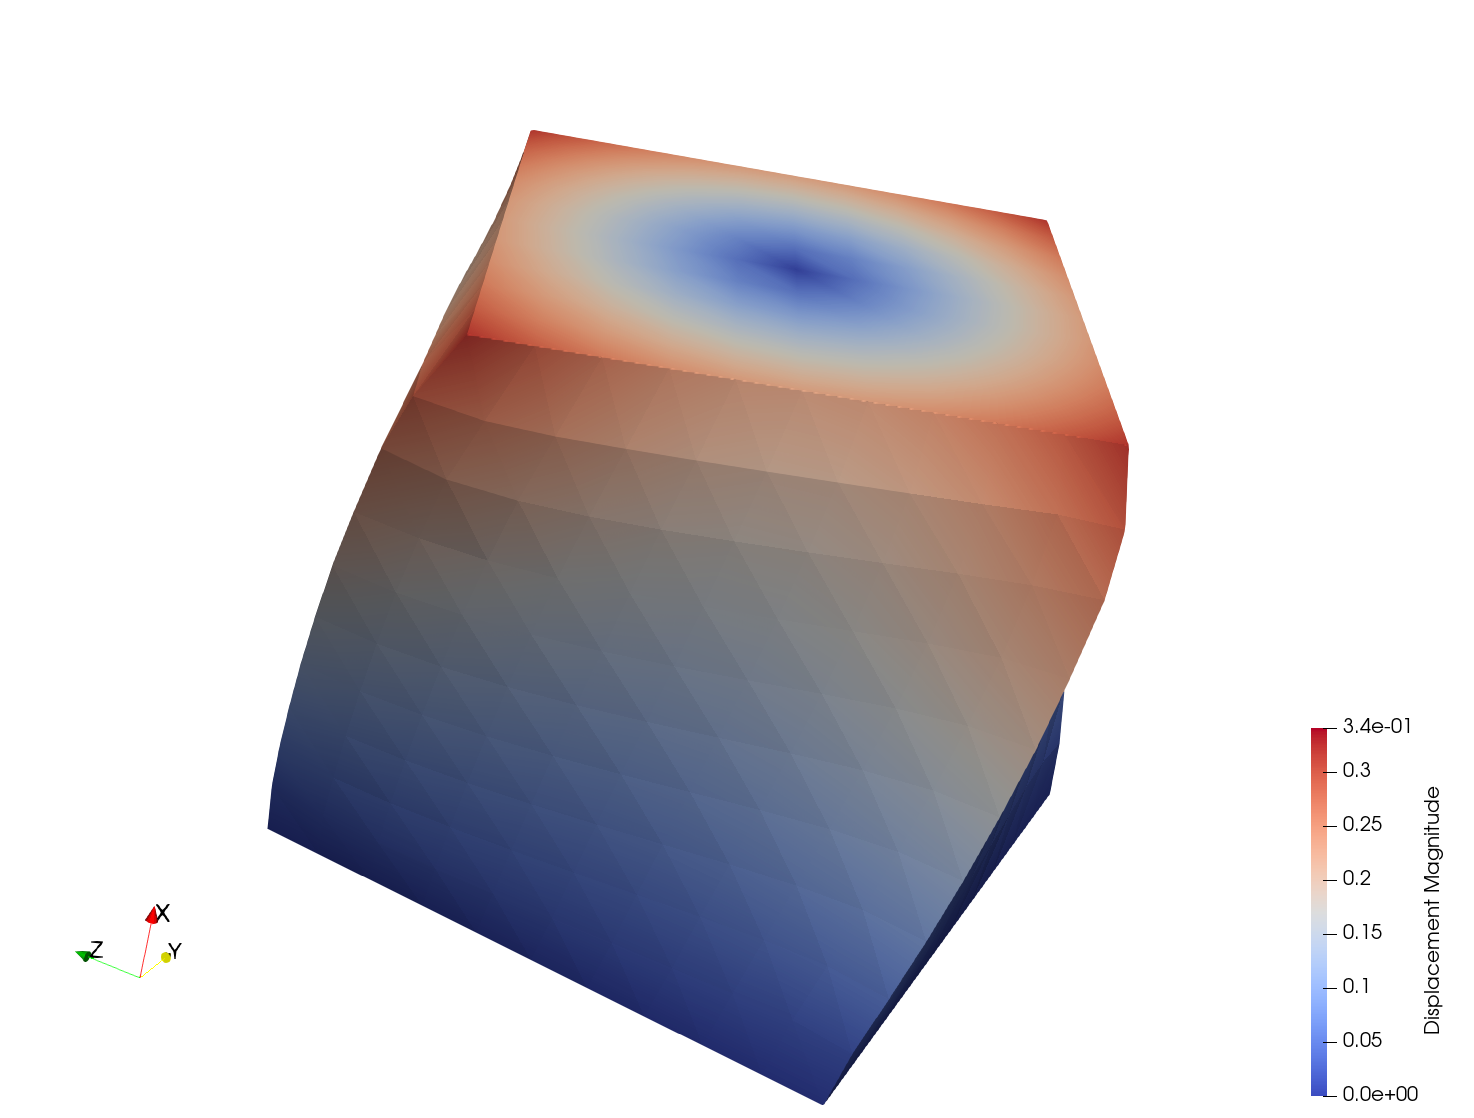
\includegraphics[width=0.49\textwidth]{./Images/MixedForm/Disp_19}
\caption{Paraview visualization of reference and final configuration of the cube subject to a twist.}
\label{FigVisual}
\end{figure*}

%===============================================================================================
%===============================================================================================
%===============================================================================================
\section{Kinematics}
\vspace{-2ex}
The displacement, $\mathbf{u}$, is the difference between points in the reference and points in the current configuration, which are denoted by $\mathbf{X}$ and $\mathbf{x}$ respectively. 
\begin{equation}\label{EqDisp}
\mathbf{u} = \mathbf{X} - \mathbf{x}
\end{equation}
By taking the gradient in the reference configuration of Eq. \ref{EqDisp}.
\begin{align*}
\pdv{\mathbf{u}}{\mathbf{X}} 
	&= \pdv{\mathbf{X}}{\mathbf{X}} - \pdv{\mathbf{x}}{\mathbf{X}} \\
\nabla \mathbf{u}
	&= \mathbf{I} - \mathbf{F}
\end{align*}
Therefore, the deformation gradient $\mathbf{F}$ maps the reference configuration to the current configuration. 
\begin{equation}\label{EqDefGrad}
\mathbf{F} = \pdv{\mathbf{x}}{\mathbf{X}} \rightarrow F_{ij} = \pdv{x_i}{X_j}
\end{equation}
and the following relationship is given, where $\mathbf{I}$ is the identity tensor. 
\begin{equation}\label{EqDefGrad2}
\mathbf{F} = \mathbf{I} + \nabla \mathbf{u} 
\end{equation}
The right Cauchy Green (CG) tensor $\mathbf{C}$ is defined as follows
\begin{equation}\label{EqRightCG}
\mathbf{C} = \mathbf{F}^T \mathbf{F}
\end{equation}
The invariants of the right CG tensor are defined as follows.
\begin{align*}
I_\mathbf{C} &= \tr \mathbf{C} \\
II_\mathbf{C} &= \frac{1}{2} (C_{kk}^2 - C_{ik} C_{ki}) \\
III_\mathbf{C} &= \det \mathbf{C} 
\end{align*}
Therefore, we can characterize the volumetric ratio between the current and reference configuration as, where we identify a relationship. 
\begin{equation}
J = \det \mathbf{F} \rightarrow J^2 = III_\mathbf{C}
\end{equation}
for an incompressible material, $J = \det \mathbf{F} = 1$. A constraint on incompressible constitutive models involves
\begin{equation}\label{EqIncompCon}
J-1 = 0
\end{equation}

%===============================================================================================
%===============================================================================================
\section{Stress Relationships}
\vspace{-2ex}
To calculate the first Piola Kirchoff (PK) stress, where $W(\mathbf{F})  = \widehat{W} (\mathbf{C})$
\begin{subequations}\label{Eq1PK}
\begin{align}
P_{ij} &= \pdv{W}{F_{ij}} \leftrightarrow \mathbf{P} = \pdv{W (\mathbf{F})}{\mathbf{F}}\\
P_{ij} &= 2 F_{ik} \pdv{\widehat{W}}{C_{jk}} \leftrightarrow \mathbf{P} = 2 \mathbf{F} \pdv{\widehat{W} (\mathbf{C})}{\mathbf{C}}
\end{align}
\end{subequations}
The Cauchy stress refers to a stress that characterizes the current or deformed configuration. 
\begin{subequations}\label{EqCauchy}
\begin{align}
\sigma_{ij} &= \frac{1}{J} F_{ik} \pdv{W (\mathbf{F})}{F_{jk}} \\
\sigma_{ij} &= \frac{2}{J} F_{ip} F_{jq} \pdv{\widehat{W} (\mathbf{C})}{C_{pq}} = \frac{1}{J} F_{ip} P_{jp}
\end{align}
\end{subequations}
We note the relationship between the Cauchy stress and the 1st Pk stress. 
\begin{align*}
\sigma_{ij} &= \frac{1}{J} F_{ik} P_{jk} \leftrightarrow \bm{\sigma} = \frac{1}{J} \mathbf{F} \mathbf{P^{T}}
\end{align*}
Where we note that $\bm{\sigma} = \bm{\sigma^T}$ because of symmetry, implying that $\mathbf{P} \mathbf{F^T} = \mathbf{F} \mathbf{P^T}$; therefore
\begin{align}\label{EqCauchyAlt}
\bm{\sigma} = \frac{1}{J} \mathbf{P} \mathbf{F^T} \leftrightarrow \sigma_{ij} = \frac{1}{J} P_{ik} F_{jk}
\end{align}
This implies that we can also write the 1st PK stress as 
\begin{align}\label{Eq1PKAlt}
\mathbf{P} = J \bm{\sigma} \mathbf{F^{-T}}
\end{align}
Using the chain rule, we can obtain a generalized expression for the 1st PK stress 
\begin{equation}\label{Eq1PKChain}
P_{ij} =  2 F_{ik} \bigg[ \pdv{\widehat{W}}{I_\mathbf{C}} \pdv{I_\mathbf{C}}{C_{kj}} 
	+ \pdv{\widehat{W}}{II_\mathbf{C}} \pdv{II_\mathbf{C}}{C_{kj}} 
	+ \pdv{\widehat{W}}{III_\mathbf{C}} \pdv{III^\mathbf{C}}{C_{kj}} \bigg]
\end{equation}
For some special cases where $J = \det \mathbf{F}$, we can state this instead as:
\begin{align}\label{Eq1PKChainIncomp}
P_{jp} &=  2 F_{jk} \bigg[ \pdv{\widehat{W}}{I_\mathbf{C}} \pdv{I_\mathbf{C}}{C_{kp}} 
	+ \pdv{\widehat{W}}{II_\mathbf{C}} \pdv{II_\mathbf{C}}{C_{kp}} \bigg]
	+ \pdv{W}{J} \pdv{J}{F_{jp}} \\
\sigma_{ij} &= \frac{1}{J} F_{ip} P_{jp}
\end{align}
The symmetric second Piola-Kirchoff stress tensor is denoted by $\mathbf{S}$
\begin{equation}\label{Eq2PK}
\mathbf{P} = \mathbf{F} \mathbf{S} \leftrightarrow P_{ij} = F_{ik} S_{kj}
\end{equation}
Where we know further that 
\begin{align}\label{Eq2PKAlt}
\mathbf{S} = 2 \pdv{\widehat{W}}{\mathbf{C}}
\end{align}
The following relationship holds, where $W(\mathbf{F})  = \widehat{W} (\mathbf{C})$
\begin{align*}
\pdv{W}{ \mathbf{F}} = 2 \mathbf{F} \pdv{\widehat{W}}{\mathbf{C}} \rightarrow \pdv{W}{F_{ij}} = 2 F_{ik} \pdv{\widehat{W}}{C_{kj}}
\end{align*}
An important relationship is included
\begin{align}\label{EqDet}
\pdv{\det \mathbf{F} }{\mathbf{F}} = \det \mathbf{F} \mathbf{F^{-T}} = J \mathbf{F^{-T}}
\end{align}

%===============================================================================================
%===============================================================================================
%===============================================================================================
\section{Strain Energy Density Function}
\vspace{-2ex}
The next section outlines some common strain energy density functions. Note that $\mu$ and $\lambda$ are Lamé Parameters and can be defined in terms of the Young's modulus, E, and Poisson's ratio $\nu$
\begin{subequations}\label{EqLame}
\begin{align}
\mu &= \frac{E}{2 (1 + \nu)} \\
\lambda &= \frac{E \nu}{(1+ \nu) (1 - 2 \nu)} 
\end{align}
\end{subequations}

%===============================================================================================
%===============================================================================================
\subsection{Compressibility}
\vspace{-1ex}
The energy density function for compressible Neo-Hookean materials is: 
\begin{equation}\label{EqStrainEnergyComp}
W (\mathbf{F})= \frac{\mu}{2} (I_\mathbf{C} - 3 - 2 \ln J) + \frac{\lambda}{2} (\ln J)^2
\end{equation}
In order to obtain the 1st PK stress, we can utilize Eq. \ref{Eq1PKChainIncomp} and use Eq. \ref{EqDet}
\begin{align*}
\mathbf{P}
	&=  2 \mathbf{F} \bigg[ \pdv{\widehat{W}}{I_\mathbf{C}} \pdv{I_\mathbf{C}}{\mathbf{C}} 
	+ \pdv{\widehat{W}}{II_\mathbf{C}} \pdv{II_\mathbf{C}}{\mathbf{C}} \bigg]
	+ \pdv{W}{J} \pdv{J}{\mathbf{F}} \\
	&=2 \mathbf{F}  \pdv{\widehat{W}}{I_\mathbf{C}} \pdv{I_\mathbf{C}}{\mathbf{C}} + \pdv{W}{J} \pdv{J}{\mathbf{F}} \\
	&= 2 \mathbf{F} \frac{\mu}{2} \pdv{I_\mathbf{C}}{\mathbf{C}} 
	+ \bigg[ \frac{\mu}{2} \pdv{(-2 \ln J)}{J} + \frac{\lambda}{2} \pdv{(\ln J)^2}{J} \bigg] \pdv{J}{\mathbf{F}} \\
	&= \mu \mathbf{F} \mathbf{I}
	+ \bigg[ \frac{\mu}{2} \pdv{(-2 \ln J)}{J} + \frac{\lambda}{2} \pdv{(\ln J)^2}{J} \bigg] \pdv{J}{\mathbf{F}} \\
	&= \mu \mathbf{F} + \bigg[ \frac{\mu}{2} \frac{-2}{J} + \frac{\lambda}{2} 2 (\ln J) \frac{1}{J} \bigg] J \mathbf{F^{-T}} \\
	&= \mu \mathbf{F} + \big[ -\mu + \lambda (\ln J) \big] \mathbf{F^{-T}} 
\end{align*}
Therefore, the 1st Piola-Kirchoff stress in the compressible case is given as, 
\begin{equation}\label{EqCompPK}
\mathbf{P} = \mu (\mathbf{F} + \mathbf{F^{-T}}) + \lambda (\ln J) \mathbf{F^{-T}}
\end{equation}


%===============================================================================================
%===============================================================================================
\subsection{Incompressibility}
\vspace{-1ex}
For an incompressible material, $J = \det \mathbf{F} = 1$; therefore, Eq. \ref{EqStrainEnergyComp} can be modified to: 
\begin{align*}
W (\mathbf{F}) &= \frac{\mu}{2} (I_\mathbf{C} - 3 - 2 \ln (1)) + \frac{\lambda}{2} (\ln (1))^2 \\
W (\mathbf{F}) &= \frac{\mu}{2} (I_\mathbf{C} - 3) 
\end{align*}
The 1st PK associated with this equation is simply
\begin{equation}\label{EqIncompPK}
\mathbf{P} = \mu \mathbf{F}
\end{equation}

One way to enforce incompressibility is to use the penalty or lagrange method of enforcing the constraint. 


%===============================================================================================
\subsubsection{Penalty Method}
\vspace{-1ex}
The penalty method enforces the constraint in Eq. \ref{EqIncompCon} with a penalty parameter $k_{pen}$.
\begin{equation}\label{EqEnergyDensityPenalty}
W(\mathbf{F}) = \frac{\mu}{2} (I_\mathbf{C} - 3) + \frac{ k_{pen}}{2} (J-1)^2
\end{equation}
This is a simple implementation that does not require expansion of the solution sub-space to include a pressure variable as in the Lagrange method, but is dependent on the penalty parameter for enforcement of the constraint. If the penalty parameter is too high, the stiffness matrix can become ill-conditioned. 

In order to obtain the 1st PK stress, we can utilize Eq. \ref{Eq1PKChainIncomp} and use Eq. \ref{EqDet}
\begin{align*}
\mathbf{P}
	&=2 \mathbf{F}  \pdv{\widehat{W}}{I_\mathbf{C}} \pdv{I_\mathbf{C}}{\mathbf{C}} + \pdv{W}{J} \pdv{J}{\mathbf{F}} \\
	&= 2 \mathbf{F} \frac{\mu}{2} \pdv{I_\mathbf{C}}{\mathbf{C}} + k_{pen}(J-1) \pdv{J}{\mathbf{F}} \\
	&= \mu \mathbf{F} \mathbf{I} + k_{pen} (J-1) J \mathbf{F^{-T}} 
\end{align*}
Therefore, the 1st PK stress in the Lagrange case of enforcing incompressibility is given as, 
\begin{equation}\label{EqPenalty1PK}
\mathbf{P} = \mu \mathbf{F} + k_{pen} (J-1) J \mathbf{F^{-T}} 
\end{equation}

%===============================================================================================
\subsubsection{Lagrange Method}
\vspace{-1ex}
To enforce incompressibility, introduce a Lagrange multiplier, $p$, which can be assumed to be a pressure-like term. 
\begin{equation}\label{EqEnergyDensityLagrange}
W(\mathbf{F}) = \frac{\mu}{2} (I_\mathbf{C} - 3) + \text{p} (J-1) 
\end{equation}
This is an exact method of enforcing incompressibility, but it requires expansion of the solution subspace to a displacement-pressure formulation. Therefore, Taylor-Hood elements have to be used for numerical stability. 

Again, to obtain the 1st PK stress, we can use Eq. \ref{Eq1PKChainIncomp}
\begin{align*}
\mathbf{P}
	&=2 \mathbf{F}  \pdv{\widehat{W}}{I_\mathbf{C}} \pdv{I_\mathbf{C}}{\mathbf{C}} + \pdv{W}{J} \pdv{J}{\mathbf{F}} \\
	&= 2 \mathbf{F} \frac{\mu}{2} \pdv{I_\mathbf{C}}{\mathbf{C}} + k_{pen}(J-1) \pdv{J}{\mathbf{F}} \\
	&= \mu \mathbf{F} \mathbf{I} + p J \mathbf{F^{-T}}
\end{align*}
Therefore,
\begin{equation}\label{EqLagrange1PK}
\mathbf{P} = \mu \mathbf{F} + \text{p} \mathbf{J} \mathbf{F^{-T}}
\end{equation}

%===============================================================================================
%===============================================================================================
%===============================================================================================
\section{Formulation}
\vspace{-2ex}

%===============================================================================================
%===============================================================================================
\subsection{Potential Energy Minimization}
\vspace{-1ex}
An alternative approach to solving static problems is to consider the minimization of potential energy.
\[ \min_{\mathbf{u} \in V} \Pi \]
where V is a suitable function space that satisfies the boundary conditions on the displacement $\mathbf{u}$. The total potential energy, $\Pi$, is given by the sum of the internal and external energy: 
\begin{align}\label{totPotEnergy}
\begin{split}
\Pi &= \Pi_{int} + \Pi_{ext} \\
	&= \bigg( \int_{\Omega} W(\mathbf{u}) dx \bigg) 
	+ \bigg( - \int_{\Omega} \mathbf{B} \cdot \mathbf{u} \, dx 
	- \int_{\partial \Omega} \mathbf{T} \cdot \mathbf{u} \, ds \bigg) 
\end{split}
\end{align}
where W is the elastic stored energy density, $\mathbf{B}$ is the body force per unit reference volume and $\mathbf{T}$ is a traction force per unit reference area. 

Minimization of the potential energy corresponds to the directional derivative of $\Pi$ being zero for all possible variations of u. (Note, minimizing $\Pi$ is equivalent to solving the balance of momentum problem.) 
\begin{equation} \label{dirDer}
L(\mathbf{u};\mathbf{v}) = D_\mathbf{v} \Pi = \frac{d \Pi (\mathbf{u} + \bm{\epsilon} \mathbf{v})}{d \bm{\epsilon}}\Bigr\rvert_{\bm{\epsilon} = 0} = 0 \indent \forall \mathbf{v} \in V
\end{equation}
If we use Newton's method, we also want to find the Jacobian of Eq. \ref{dirDer}
\begin{equation} \label{JacDirDer}
a(\mathbf{u};d\mathbf{u},\mathbf{v}) = D_{d\mathbf{u}} L = \frac{dL(\mathbf{u}+ \bm{\epsilon} \, d\mathbf{u}; \mathbf{v})}{d \bm{\epsilon}} \Bigr\rvert_{\bm{\epsilon} = 0}
\end{equation}

%===============================================================================================
%===============================================================================================
\subsection{Strong to Weak Form}
\vspace{-1ex}
This is another notation commonly used, where a capital index is used to indicate the referential configuration and a lowercase index is used to indicate the current configuration. The 1st PK stress is a tensor that represents both the referential and the current configuration, but the 2nd PK stress is a tensor purely in the referential configuration. The mechanical equilibrium equation is given as: 
\begin{subequations}\label{EqEqm}
\begin{align}
\nabla_X \mathbf{P} + \mathbf{B} &= \mathbf{0} \quad \text{in } \Omega_0 \\
\mathbf{u} &= \mathbf{u_0} \quad \text{on } \Gamma_D \\
\mathbf{P} \cdot \mathbf{N} &= \mathbf{T} \quad \text{on } \Gamma_N 
\end{align}
\end{subequations}
where the Dirichlet and Neumann boundary conditions are given on there respective boundaries, and the body force and traction force are defined as $\mathbf{B}$ and $\mathbf{T}$ respectively. The mechanical equilibrium equation can be written in indicial notation: 
\begin{equation}\label{EqEqmInd}
P_{iJ,J} + B_i = 0 \rightarrow \pdv{P_{iJ}}{X_J} + B_i = 0 
\end{equation}
Take Eq. \ref{EqEqmInd} and multiply by a test function, $\mathbf{v} = v_i \mathbf{e_i}$
\begin{align}\label{EqBefInt}
\begin{split}
\pdv{P_{iJ}}{X_J} \mathbf{e_i} \cdot v_j \mathbf{e_j} &= - B_i \mathbf{e_i} \cdot v_j \mathbf{e_j} \\
\pdv{P_{iJ}}{X_J} v_j \delta_{ij} &= - B_i v_j \delta_{ij} \\
\pdv{P_{iJ}}{X_J} v_i &= - B_i v_i \quad \text{Integrate over domain} \\
\int_{\Omega_o} \pdv{P_{iJ}}{X_J} v_i dV &= - \int_{\Omega_o} B_i v_i dV
\end{split}
\end{align}
Use integration by parts: 
\begin{align*}
(fg)' = f'g + f g' \rightarrow f'g &= (fg)' - f g' \\
			\pdv{P_{iJ}}{X_j} v_i &= (P_{iJ} v_i)_{,J} - P_{iJ} v_{i,J}
\end{align*}
Substitute into Eq. \ref{EqBefInt}:
\begin{align*}
\int_{\Omega_o} (P_{iJ} v_i)_{,J} dV - \int_{\Omega_o} P_{iJ} v_{i,J} dV &= - \int_{\Omega_o} B_i v_i dV \quad \text{Use divergence theorem} \\
\int_{\partial \Omega_o} P_{iJ} N_J v_i dS - \int_{\Omega_o} P_{iJ} v_{i,J} dV &= - \int_{\Omega_o} B_i v_i dV \quad \text{Recognize traction } P_{iJ} N_J = T_i\\
\int_{\partial \Omega_o} T_i v_i dS - \int_{\Omega_o} P_{iJ} v_{i,J} dV &= - \int_{\Omega_o} B_i v_i dV \quad \text{Rearrange} \\
\int_{\Omega_o} P_{iJ} v_{i,J} dV &= \int_{\Omega_o} B_i v_i dV + \int_{\partial \Omega_o} T_i v_i dS 
\end{align*}
Rewrite in direct notation to obtain weak form: 
\begin{equation}\label{EqWeakFormDirect}
 \int_{\Omega_o} \mathbf{P} : \text{Grad}(\mathbf{v}) \, dV = \int_{\Omega_o} \mathbf{B} \cdot \mathbf{v} \, dV + \int_{\Gamma_N} \mathbf{T} \cdot \mathbf{v} \, dS
\end{equation}
Finally, in order to enforce incompressibility we use the constraint equation Eq. \ref{EqIncompCon}, where we can multiply this with a scalar test function
\begin{align*}
 J - 1 &= 0 \\ 
\int_{\Omega} (J-1) \tau \, dV &= 0. 
\end{align*}
Therefore the weak forms are as listed in Eq. \ref{EqWeakFormTotal}
\begin{subequations}\label{EqWeakFormTotal}
\begin{align}
 \int_{\Omega_o} \mathbf{P} : \text{Grad}(\mathbf{v}) \, dV &= \int_{\Omega_o} \mathbf{B} \cdot \mathbf{v} \, dV + \int_{\Gamma_N} \mathbf{T} \cdot \mathbf{v} \, dS \\
\int_{\Omega_o} (J - 1) \tau \, dV &= 0
\end{align}
\end{subequations}
The bilinear and linear form can be stated where we have two test functions
\begin{equation*}
a \big( (\mathbf{u}, p),( \mathbf{v}, \tau) \big) = L \big( (\mathbf{v}, \tau) \big) \indent \forall (\mathbf{v}, \tau) \in \Sigma_0 \times V 
\end{equation*}
Therefore with Eq. \ref{EqWeakFormTotal}, we have the bilinear and linear forms: 
\begin{equation}\label{EqBilinear}
a \big( (\mathbf{u}, p),( \mathbf{v}, \tau) \big) 
	= \int_{\Omega_o} \big( \mathbf{P} : \text{Grad}(\mathbf{v}) 
	+ (J-1) \tau \big) \, dV
\end{equation}
\begin{equation}\label{EqLinear}
L \big( (\mathbf{v}, \tau) \big) 
	= \int_{\Omega_o} \mathbf{B} \cdot \mathbf{v} \, dV 
	+ \int_{\partial \Omega_o} \mathbf{T} \cdot \mathbf{v} \, dS
\end{equation}
The bilinear and linear form (Eq. \ref{EqBilinear} and \ref{EqLinear}) can also be combined into one statement, where we solve for two unknowns, displacement ($\mathbf{u}$) and hydrostatic pressure (p). 
\begin{equation}
a \big( (\mathbf{u}, p),( \mathbf{v}, \tau) \big) - L \big( (\mathbf{v}, \tau) \big) 
	= \int_{\Omega_o} \big( \mathbf{P} : \text{Grad}(\mathbf{v}) 
	+ (J-1) \tau \big) \, dV
	- \int_{\Omega_o} \mathbf{B} \cdot \mathbf{v} \, dV 
	- \int_{\partial \Omega_o} \mathbf{T} \cdot \mathbf{v} \, dS
\end{equation}

%===============================================================================================
%===============================================================================================
%===============================================================================================
\section{FEniCS Implementation}
\vspace{-2ex}

There are three codes provided, the first one demonstrates the energy minimization formulation for the displacement only formulation, with two choices of model, 1) a compressible neo-Hookean model and 2) an incompressible penalty formulation. The second code demonstrates a penalty formulation with an explicit weak form. The third code demonstrates a Lagrange formulation with an explicit weak form. \\
{\fontfamily{qcr}\selectfont
HyperelasticEnergy.py \\
HyperelasticDispForm.py \\ 
HyperelasticMixedForm.py \\ \\
}
The domain is a unit cube where the x-direction faces towards the right and the y-direction is upwards by default in Paraview 
\[ \Omega = (0,1) \times (0,1) \times (0,1)\] 
The left hand side is completely fixed, while a twist is provided to the right side of the cube. The function for the twist is specified in Eq. \ref{EqTwistFcn}, which is why y and z direction are specified and the x-direction is zero.
\begin{equation}\label{EqTwistFcn}
\mathbf{u} = 
	\bigg[ 0, 
	s \bigg(\frac{1}{2} + (y-\frac{1}{2}) \cos \theta - (z-\frac{1}{2}) \sin \theta - y \bigg),
	s \bigg( \frac{1}{2} + (y-\frac{1}{2}) \sin \theta - (z-\frac{1}{2}) \cos \theta - z \bigg) 
	\bigg] 
\end{equation}
Certain parameters of this equation can be increased over the course of the simulation, $s$ is a scaling parameter, and $\theta$ is the angle of the twist provided. The first parameters provided  \\
{\fontfamily{qcr}\selectfont
r = Expression(("scale*0.0", \\
\indent "scale*(.5 + (x[1] - .5)*cos(theta) - (x[2] - .5)*sin(theta) - x[1])", \\
\indent "scale*(.5 + (x[1] - .5)*sin(theta) + (x[2] - .5)*cos(theta) - x[2])"), \\
\indent scale = 0, theta = 0, degree=2) \\ 
 }
where {\fontfamily{qcr}\selectfont scale} and {\fontfamily{qcr}\selectfont theta} can be adjusted in the loop according to \\
{\fontfamily{qcr}\selectfont 
RampArray = np.linspace(0, 0.5, TotSteps)  \\
ThetaArray = np.linspace(0, pi/3, TotSteps) \\ \\
}
Note the general way to declare aspects of the expression \\
{\fontfamily{qcr}\selectfont 
Expression("x+y", x = \#, y = \#, degree = \#) \\ \\
} 
The behavior of the FEniCS Form Compiler, FFC, can be adjusted by prescribing various parameters. Use the UFL Analyzer and Compiler System, UFLACS, which is the backend of FFC. Changes were made to parse in user parameters: \\
{\fontfamily{qcr}\selectfont
parameters.parse() \\
UserPar = Parameters("user") \\
UserPar.add("TotSteps", 20) \\
UserPar.parse() \\ \\
}
From there, the following syntax can be used to define the parameter: \\
{\fontfamily{qcr}\selectfont
TotSteps = UserPar["TotSteps"]   \\ \\
}
Some parameters can be defined using the {\fontfamily{qcr}\selectfont Constant } syntax, which is used in order to avoid re-generation of C++ code when changing model parameters. \\
{\fontfamily{qcr}\selectfont
mu = Constant(E/(2*(1 + nu))) \\ \\
}
Create a unit cube with 25 (24 + 1) vertices in one direction and 17 (16 + 1) vertices in the other two directions: \\
{\fontfamily{qcr}\selectfont
mesh = UnitCubeMesh(24, 16, 16) \\ \\
}
Note: C++ syntax is used in the `CompiledSubDomain` function since the function will be automatically compiled into C++ code for efficiency. \\ 
{\fontfamily{qcr}\selectfont
left =  CompiledSubDomain("near(x[0], side) \&\& on\_boundary", side = 0.0) \\ \\
}
The Dirichlet (essential) boundary conditions are constraints on the function space V. Use the following definitions for the boundary conditions, where we have Dirichlet boundary conditions on the left and right surface of the cube and a potential Neumann boundary condition dependent on whether traction is specified.
\[ \Gamma_{D_0} = 0 \times (0,1) \times (0,1) \]
\[ \Gamma_{D_1} = 1 \times (0,1) \times (0,1) \]


%===============================================================================================
%===============================================================================================
\subsection{Displacement Formulation}
\vspace{-1ex}
The displacement formulation only requires the definition of a function space with continuous piecewise linear vector polynomials. Note that VectorFunctionSpace creates a function space of vector fields. The dimension of the vector field (the number of components) is assumed to be the same as the spatial dimension, unless otherwise specified. \\
{\fontfamily{qcr}\selectfont
V = VectorFunctionSpace(mesh, "Lagrange", 1) \\ \\
}
As another option, an additional tensor space, where DG = Discontinuous Galerkin, can be defined which is for projection of the stress. DG0 space refers to a scalar space for projection of $J=\det \mathbf{F}$ to determine how closely incompressibility is being maintained. \\
{\fontfamily{qcr}\selectfont
T\_DG0 = TensorFunctionSpace(mesh, "DG", 0) \\ 
DG0 = FunctionSpace(mesh, "DG", 0) \\ \\
}
In the {\fontfamily{qcr}\selectfont HyperelasticEnergy.py} file, two strain energy density equations are defined based on Eq. \ref{EqStrainEnergyComp} and Eq. \ref{EqEnergyDensityPenalty}, where the user parameter {\fontfamily{qcr}\selectfont Model} determines which equation is used (same for the equations for the 1st PK Stress).  The total potential energy can be set up as follows,\\
{\fontfamily{qcr}\selectfont 
Pi = psi(Ic,J)*dx - dot(B, u)*dx - dot(T, u)*ds \\
WF = derivative(Pi, u, v) \\
Jc = derivative(WF, u, du)  \\  \\
}
In {\fontfamily{qcr}\selectfont HyperelasticDispForm}, the weak form is written explicitly for the penalty method of enforcing incompressibility. For the first term, the algorithm will estimate the polynomial degree and use many Gauss points to approximate the integral. Using the line {\fontfamily{qcr}\selectfont (metadata={"quadrature\_degree": 4})} allows us to specify the number of Gauss points explicitly. In this case, the weak form looks like: \\
 {\fontfamily{qcr}\selectfont 
WF = (inner(P(F), grad(v)))*dx(metadata={"quadrature\_degree": 4}) \\
\indent \indent - dot(B, v)*dx - dot(T, v)*ds \\ \\
}
\noindent A for loop is set up to increase the {\fontfamily{qcr}\selectfont scale} and  {\fontfamily{qcr}\selectfont theta} parameter within the expression. Read in the {\fontfamily{qcr}\selectfont numpy} library to create a linearly spaced array. \\
{\fontfamily{qcr}\selectfont 
RampArray = np.linspace(0, 0.5, TotSteps) \\ 
ThetaArray = np.linspace(0, pi/3, TotSteps) \\ 
for (Step, Scale) in enumerate(RampArray): \\
\indent solve(WF == 0, u, bcs, J=Jc) \\
\indent r.scale = Scale \\
\indent r.theta = ThetaArray[Step] \\ \\
}
Post-processing is also carried out where parameters of interest are saved to a text file. In this case, we save the step number, the scale parameter in the expression, and each direction of displacement at the point, (1,1,1). \\
{\fontfamily{qcr}\selectfont 
PostProc = np.zeros((TotSteps, 5)) \\
for (Step, Scale) in enumerate(RampArray): \\
\indent PostProc[Step] = np.array([Step, Scale, \\
\indent\indent\indent\indent\indent\indent\indent\indent\indent\indent\indent\indent
u(1,1,1)[1], u(1,1,1)[2], DetF(1,1,1) ]\\
\indent np.savetxt(SaveDir + SimPar + '/PostProc.txt', PostProc) \\ \\
}
Saving variables like this to a text file can allow for easy comparison of displacements (or other parameters of interest).

%===============================================================================================
%===============================================================================================
\subsection{Mixed Formulation}
\vspace{-1ex}
There are two unknowns in our formulation, displacement and hydrostatic pressure, $\mathbf{u}, \, p$ Therefore, define a vector space of degree 2 for displacement and degree 1 for pressure. \\
{\fontfamily{qcr}\selectfont
V\_CG2 = VectorElement("Lagrange", mesh.ufl\_cell(), 2) \\
V\_CG1 = FiniteElement("Lagrange", mesh.ufl\_cell(), 1) \\ \\
}
Taylor-Hood elements, {\fontfamily{qcr}\selectfont TH}, are elements defined where one vector space is one degree higher than the other. These type of elements are stable for this formulation. In our case, the vector space for displacement is one degree higher than that of pressure: \\ 
{\fontfamily{qcr}\selectfont
TH = MixedElement([V\_CG2, V\_CG1]) \\
V  = FunctionSpace(mesh, TH) \\ \\
}
The only difference from the displacement formulation involves splitting the test functions and the function into the displacement and pressure. Note that this is a shallow copy not a deep copy. An example of a deep copy is shown within the for loop.\\
{\fontfamily{qcr}\selectfont
(v\_u, v\_p) = split(v) \\
(u, p) = split(w) \\ \\
}
The weak form has the additional equation included for enforcing incompressibility. Note that body force and traction are constants, the automatic inference algorithm will use 1 Gauss point to represent those integrals. If we don't specify the quadrature degree, a warning will appear about computational time: \\ 
{\fontfamily{qcr}\selectfont
WF = (inner(P(F), grad(v\_u)) \\
\indent \indent + inner(J-1., v\_p))*dx(metadata={"quadrature\_degree": 4}) \\
\indent \indent - dot(B, v\_u)*dx - dot(T, v\_u)*ds \\ \\
}
In this specific formulation, different solver parameters are setup. \\
{\fontfamily{qcr}\selectfont
J\_o = derivative(WF, w, du) \\
varproblem = NonlinearVariationalProblem(WF, w, bcs, J=J\_o) \\
for (Step, Scale) in enumerate(RampArray): \\
\indent     solver.solve() \\
\indent     (u, p) = w.split() \\ \\
}
This split function is a deep copy, which is important for saving the solution for visualization. A post-processing file is also created in the same manner as the other codes to provide consistency in results. 

\section{Results}
\vspace{-2ex}
The code {\fontfamily{qcr}\selectfont PostProc.py} accesses the text files of interest. The displacement in the $y$ and $z$ direction at point $[1,1,1]$ is tracked and plotted next to the expression applied through a Dirichlet boundary condition. The displacement results for all these formulations, in order, are given in Fig. \ref{FigFormComparison}. The comparison of the displacement results from all the formulations shows that they produce results consistent to each others. They also display some deviation from the applied expression.

\begin{figure*}[!htb]
\centering
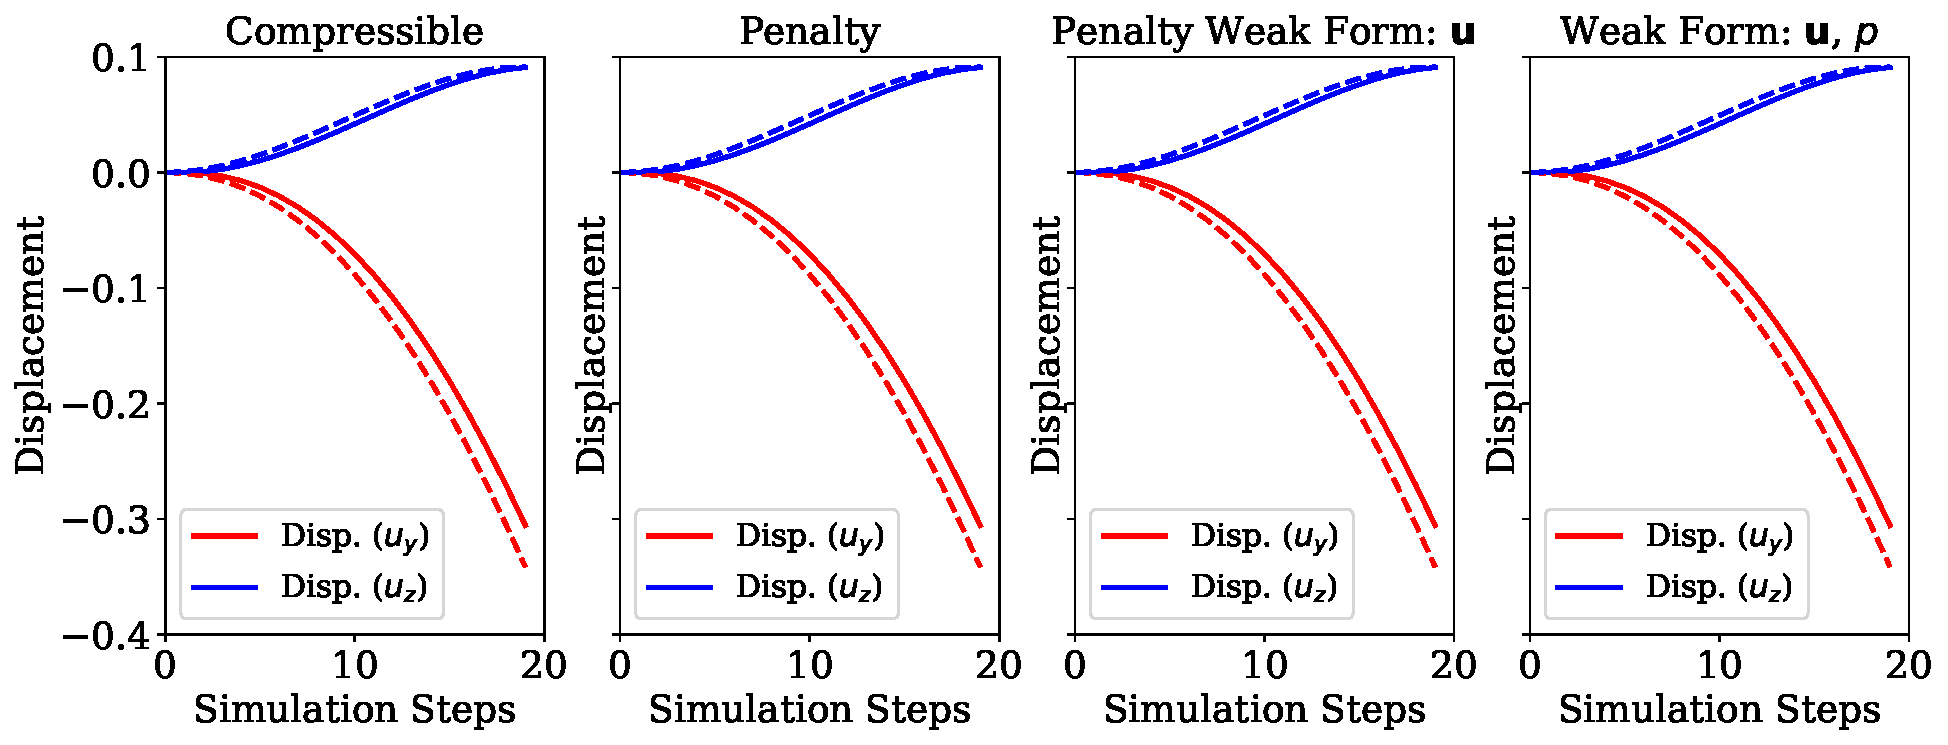
\includegraphics[width=\textwidth]{./Images/FormComp_Disp_Nu_049}
\caption{Expression applied is demonstrated with a dashed line while displacement results are displayed with a solid line. A) Comparison of results from HyperelasticEnergy.py where different constitutive models are applied in a displacement-only formulation. B) Comparison of displacement (penalty) and displacement pressure (Lagrange) formulation results where the weak form is explicitly defined, where $\nu = 0.49$.}
\label{FigFormComparison}
\end{figure*}

While the displacement results are consistent, the incompressibility parameter $J=det \mathbf{F}$ is not necessarily enforced at $J=1$. First, we can examine the results from {\fontfamily{qcr}\selectfont HyperelasticDispForm.py} plotted in Fig. \ref{FigWeakFormU_J}A, where we can see how incompressibility is more closely maintained at 1 as the Poisson's ratio increases. Next, we can compare this result to the energy minimization formulation in Fig. \ref{FigWeakFormU_J}B, where we see identical results for the same mesh parameters, $N_x = N_y = N_z = 10$

\begin{figure*}[!htb]
\centering
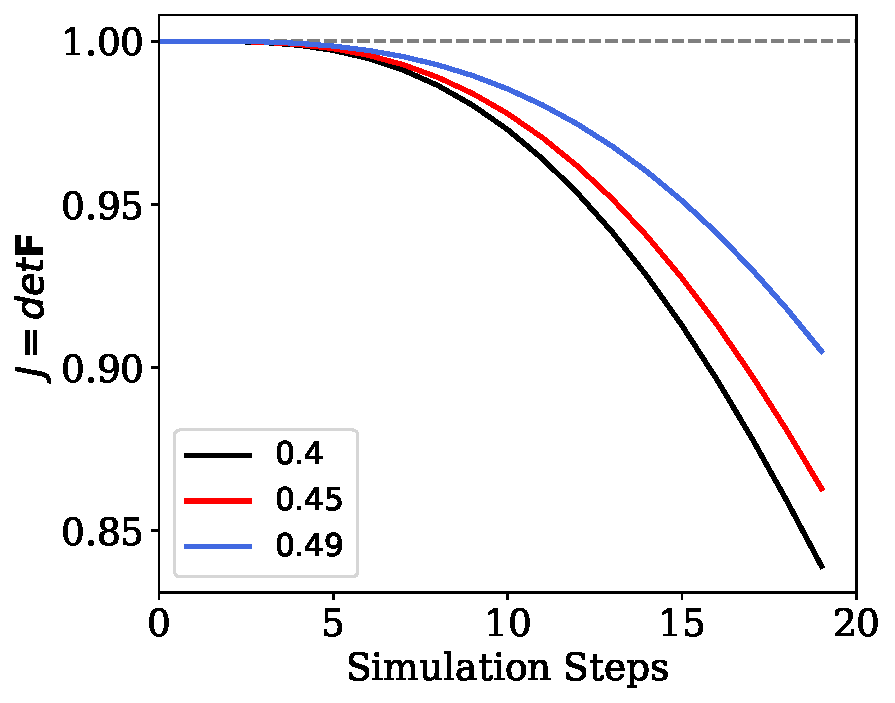
\includegraphics[width=0.49\textwidth]{./Images/EnergyPenalty_J_Nu_v}
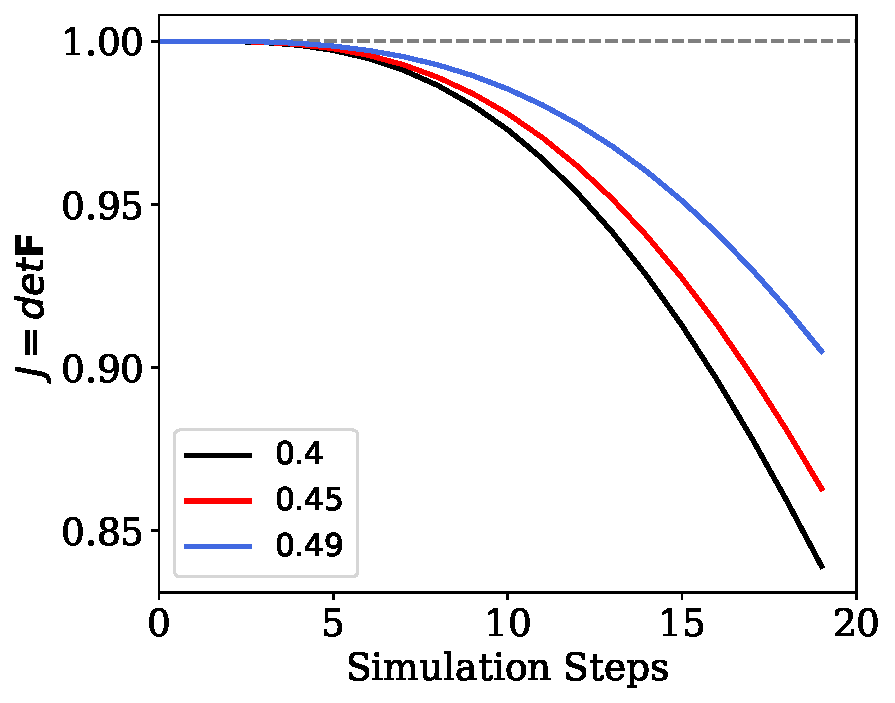
\includegraphics[width=0.49\textwidth]{./Images/WeakFormU_J_Nu_v}
\caption{Incompressibility results at point (1,1,1) of the cube. A) Energy formulation B) Plotted for varying Poisson's ratio for the penalty formulation with explicit weak form. Higher Poisson's ratio leads to a higher bulk modulus which maintains the incompressibility constraint more strictly. B) Comparison of incompressibility constraints for different formulations. First two listed work by potential energy minimization, and last two listed contain the explicit weak form statement. }
\label{FigWeakFormU_J}
\end{figure*}

\newpage

Fig. \ref{FigFormComp} demonstrates the evolution of the incompressibility constraint where $\nu = 0.49$ among the different formulations. As expected, the compressible formulation does not enforce $J = 1$, and the Lagrange formulation holds the incompressibility constraint the most strictly. 

\begin{figure*}[!htb]
\centering
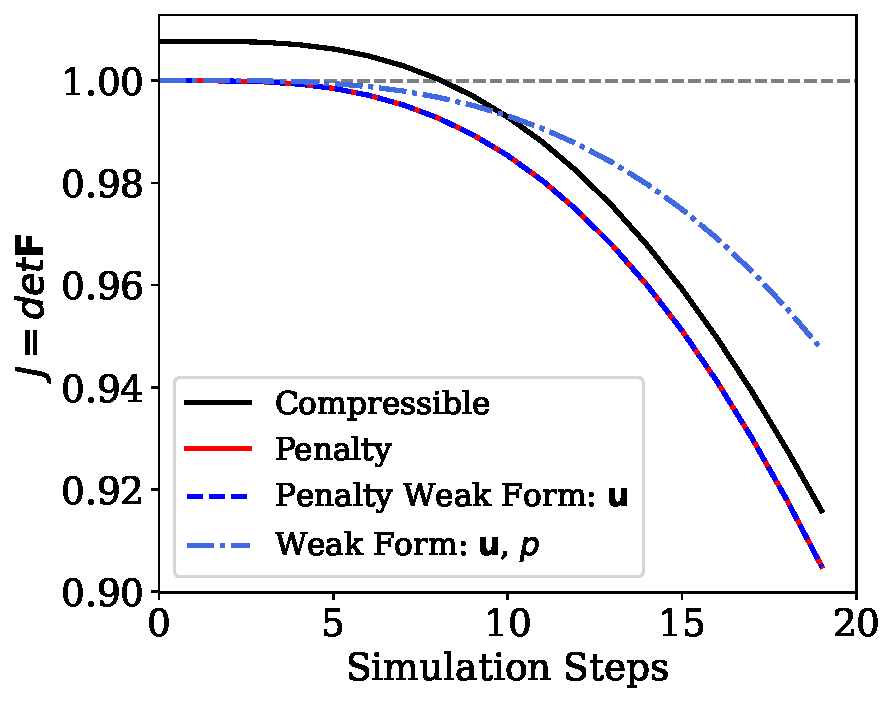
\includegraphics[width=0.75\textwidth]{./Images/FormComp_J_Nu_049}
\caption{Comparison of incompressibility constraints for different formulations on a mesh where $N_x = N_y= N_z = 10$. First two listed work by potential energy minimization, and last two listed contain the explicit weak form statement. }
\label{FigFormComp}
\end{figure*}






 



\end{document}
